% Status info:
% M. Gates	2006-2009
% A. Wolf	2011-2014
% B. Gerdes	2013
% Additions inserted from wiki 2015-12-26
% Content OK for 0.12.4.
% 2016-04 GZ started restructuring
% TODO: typo&grammar check

% \chapterimage{chapter-t2-bg} % Chapter heading image now set in guide.tex

\chapter{The User Interface}
\label{ch:gui}


This chapter describes the dialog windows which can be accessed from the left menu bar.

Most of Stellarium's settings can be changed using the configuration
window and the view window. To open the configuration window, click the
button on the left side toolbar or press \key{F2}. To open the view window
click the button on the left side toolbar or press \key{F4}.

Some options may only be configured by editing the configuration file.
See \ref{sec:ConfigurationFile} The Main Configuration File for more
details.


\newFeature{0.15} You can drag the
windows around, and the position will be used again when you restart
Stellarium. If this would mean the window is off-screen (because you
start in windowed mode, or with a different screen), the window will
be moved so that at least a part is visible.


\section{Setting the Date and Time}
\label{sec:gui:date}

\begin{figure}[h]
\centering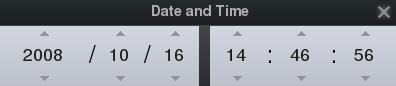
\includegraphics{date_and_time_dialog}
\caption{Date and Time dialog}
\label{fig:gui:date}
\end{figure}

In addition to the time rate control buttons on the main toolbar, you
can use the date and time window (open with the ``clock'' button or \key{F5}) to set the simulation time. The values
for year, month, day, hour, minutes and seconds may be modified by
typing new values, by clicking the up and down arrows above and below
the values, and by using the mouse wheel.

\subsection{Julian Day Number}
\label{sec:gui:date:julian}

In the 19th century, European astronomers have introduced the use of
Julian Day numbers (invented around the time of the Gregorian calendar
reform). This is a simple continuous day count starting on January 1, -4712
(4713 BC). There are no years, months etc., and the integral day
number switches at noon, so during a single night of observation (in
Europe) the date never changes. 

The fractional part of the number is just the fraction of day that has
elapsed since last noon. Given that a day has 86400~seconds, we should
give a JD with 5 decimal places to capture the nearest second.

This causes a problem for modern computers: even a ``double precision
float'' can keep only about 13 decimal places. More than 2.4 million
days have passed, so that e.g. January 1, 2000, 12:00UT is 2451545.0,
which is an accurately storable number with 7 decimal places, but 12:34:56UT is computed as
2451545.02426. A more accurate result would yield
2451545.024259259259... So, for a field where sub-second accuracy
became crucial like spacecraft operations, the \indexterm{Modified
  Julian Date} (MJD) has been introduced. It is simply
\begin{equation}
  \label{eq:MJD}
  MJD=JD-2400000.5. 
\end{equation}
This means, days start at midnight, and the (constant, in our era)
decimal places of the ``big numbers'' at the begin of the number have
been traded in for more decimal places at the end. 

Don't put your expectations too high when you see MJD displayed:
Stellarium uses JD for internal timekeeping, and Stellarium's display
of MJD is simply computed from it. So you cannot set temporal
increments smaller than a second, and it hardly would make sense to
expect more.

\section{Setting Your Location}
\label{sec:gui:location}

\begin{figure}[htb]
\centering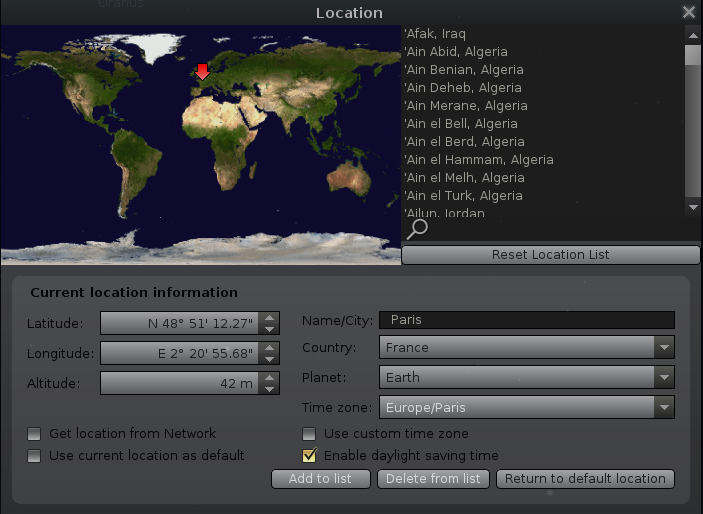
\includegraphics[scale=0.68]{location_dialog}
\caption{Location window}
\label{fig:gui:location}
\end{figure}

The positions of the stars in the sky is dependent on your location on
Earth (or other planet) as well as the time and date. For Stellarium to
show accurately what is (or will be/was) in the sky, you must tell it
where you are. You only need to do this once -- Stellarium can save your
location so you won't need to set it again until you move.

\newFeature{0.13.1}
After installation, Stellarium uses a lookup service which tries to
find your approximate location based on the IP address you are
using. This seems very practical, but if you feel this causes privacy
issues, you may want to switch this feature off. You should consider
switching it off on a computer which does not move, to save network
bandwidth.

To set your location more accurately, or if the lookup service fails,
press \key{F6} to open the location window. There are a few ways you
can set your location:

\begin{enumerate}
\item Just click on the map.
\item Search for a city where you live using the search edit box at
  the top right of the window, and select the right city from the
  list.
\item Click on the map to filter the list of cities in the vicinity of
  your click, then choose from the shortlist.
\item Enter a new location using the longitude, latitude and other
  data.
\end{enumerate}

Once you're happy that the location is set correctly, click on the ``use
as default'' checkbox, and close the location window.



\section{The Configuration Window}
\label{sec:gui:configuration}

The configuration window contains general program settings, and many
other settings which do not concern specific display options. Press
the tool button or \key{F2} to open.

\begin{figure}[h]
\centering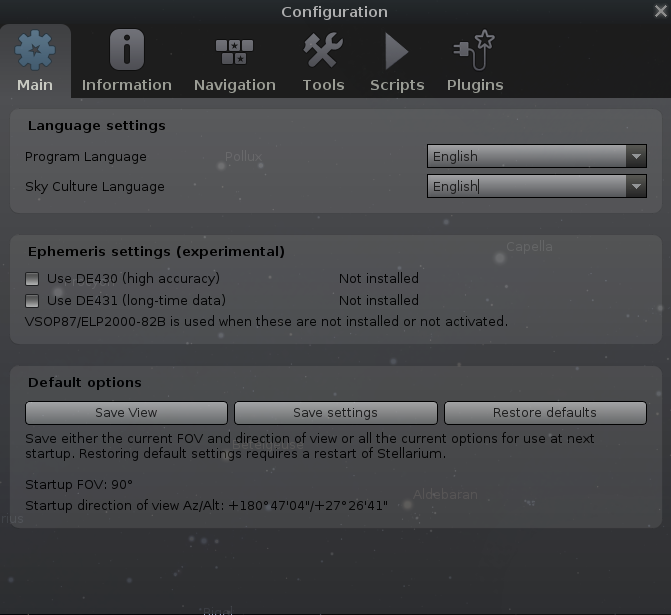
\includegraphics[scale=0.68]{config_dialog_main_tab}
\caption{Configuration Window: Main Tab}
\label{fig:gui:configuration:main}
\end{figure}

The Main tab in the configuration window provides controls for changing
the program language, how much information is shown about selected sky
objects, and provides a button for saving the current program
configuration.

\begin{figure}[h]
\centering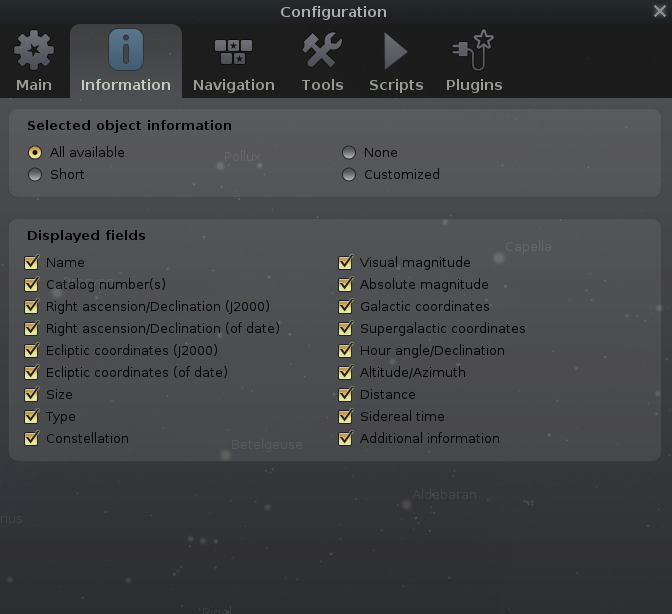
\includegraphics[scale=0.68]{config_dialog_info_tab}
%\caption{Figure caption}
\caption{Configuration Window: Information Tab}
\label{fig:gui:configuration:info}
\end{figure}

The Information tab allows you to set the type and amount of information
displayed on a selected object.
\begin{itemize}
\item Ticking or unticking the relevant boxes will control this.
\item The information displays in various colours depending on the type and
level of the stored data
\end{itemize}

\begin{figure}[h]
\centering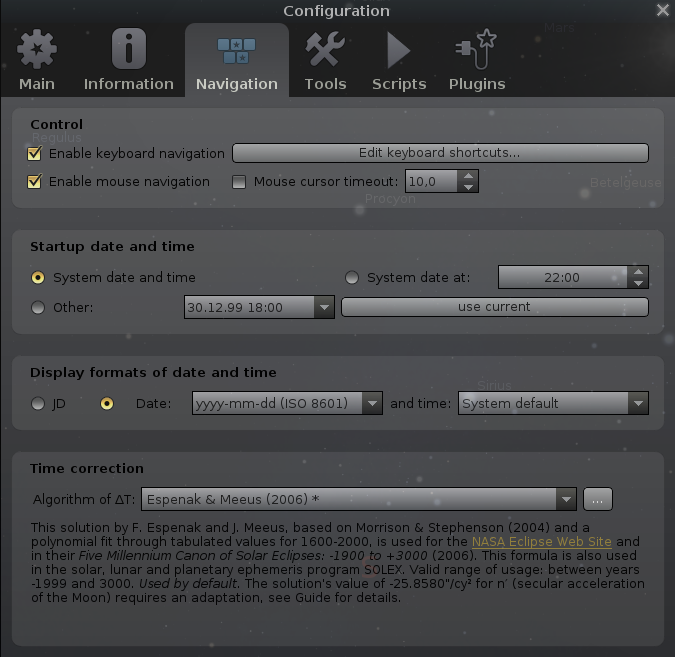
\includegraphics[scale=0.68]{config_dialog_navigation_tab}
%\caption{Figure caption}
\label{fig:gui:configuration:nav}
\end{figure}

The Navigation tab allows for enabling/disabling of keyboard shortcuts
for panning and zooming the main view, and also how to specify what
simulation time should be used when the program starts:

\begin{description}
\item[System date and time]: Stellarium will start with
  the simulation time equal to the operating system clock.
\item[System date at]: Stellarium will start with the
  same date as the operating system clock, but the time will be fixed at
  the specified value. This is a useful setting for those people who use
  Stellarium during the day to plan observing sessions for the upcoming
  evening.
\item[Other]: some fixed time can be chosen which will
  be used every time Stellarium starts.
\end{description}

\begin{figure}[h]
\centering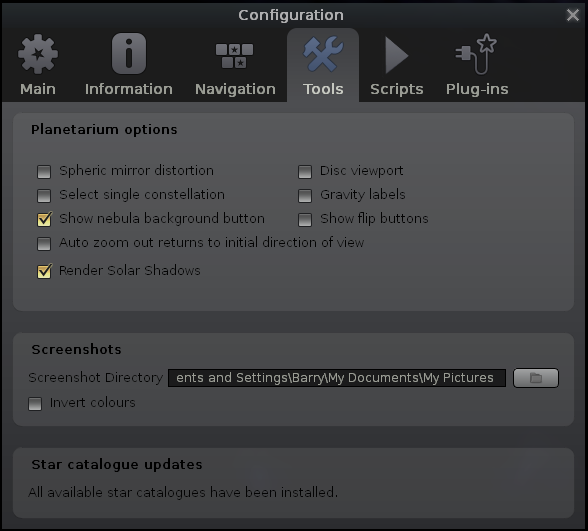
\includegraphics[scale=0.68]{config_dialog_tools_tab}
%\caption{Figure caption}
\end{figure}

The Tools tab of the configuration window contains miscellaneous utility
features:

\begin{description}
\item[Show flip buttons] When enabled, two buttons will be added to
  the main tool-bar which allow the main view to be mirrored in the
  vertical and horizontal directions. This is useful when observing
  through telecopes which may cause the image to be mirrored.
\item[Spheric mirror distortion] This option pre-warps the main view
  such that it may be projected onto a spherical mirror using a
  projector. The resulting image will be refected up from the spherical
  mirror in such a way that it may be shone onto a small planetarium
  dome, making a cheap planetarium projection system.
\item[Disc viewport] This option limits masks the main view
  producing the effect of a telescope eyepiece. It is also useful when
  projecting Stellarium's output with a fish-eye lens planetarium
  projector.
\item[Gravity labels] This option makes labels of objects in the
  main view align with the nearest horizon. This means that labels
  projected onto a dome are always alighned properly.
\item[Auto zoom out returns to initial field of view] When enabled,
  this option changes the behaviour of the zoom out key
  (\textbackslash{}) so that it resets the initial direction of view in
  addition to the field of view.
\end{description}

\subsection{The Scripts Tab}
\label{sec:gui:scripts}


\begin{figure}[h]
\centering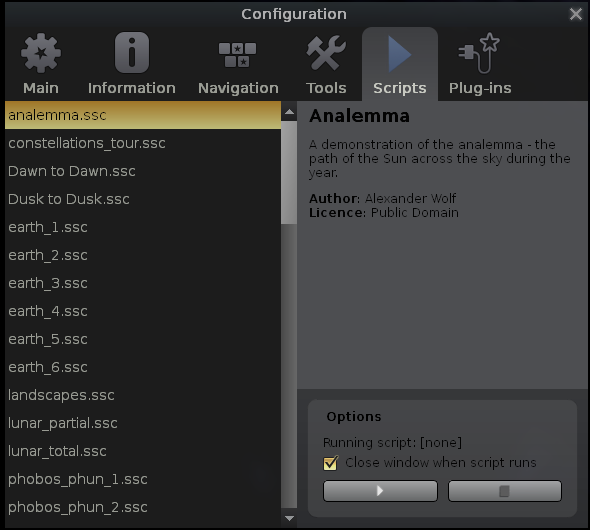
\includegraphics[scale=0.68]{config_dialog_scripts_tab}
%\caption{Figure caption}
\label{fig:gui:scripts}
\end{figure}

The Scripts tab allows the selection of pre-assembled scripts bundled
with Stellarium that can be run. This list can be expanded by your own
scripts as required. See
\ref{sec:FilesAndDirectories:DirectoryStructure} where to store your
own scripts.

When a script is selected it can be run by pressing the arrow button
and stopped with the stop button. With some scripts the stop button is
inhibited until the script is finished. %% TODO: EXPLAIN HOW?

Scripts that use sound or embedded videos will need a version of
Stellarium compiled at compile time with multimedia support
enabled. It must be pointed out here that sound or video codecs
available depends on the sound and video capabilities of you computer
platform and may not work.


\subsection{The Plugins Tab }
\label{sec:gui:plugins}


\begin{figure}[h]
\centering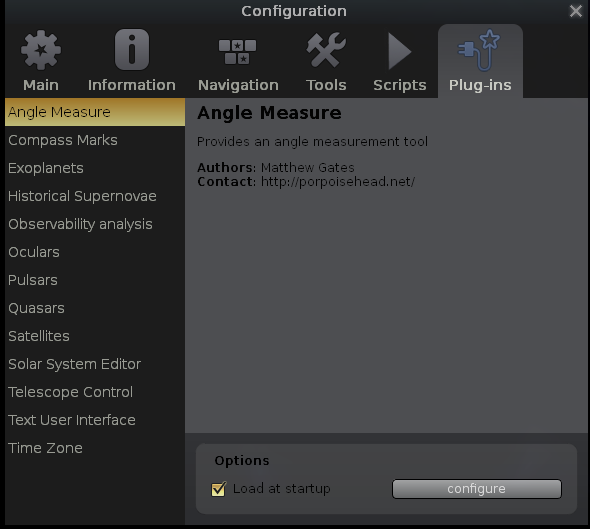
\includegraphics[scale=0.68]{config_dialog_plugins_tab}
\caption{Configuration Window: Plugins}
\label{fig:gui:plugins}
\end{figure}

Plug ins need to be enabled at start up to be available
as shown on the bar. This allows for the selection of the plugins that
you wish to be enabled at this time:

\section{The View Settings Window}\label{the-view-settings-window}

The View settings window controls many display features of Stellarium
which are not available via the main toolbar.

\subsection{Sky Tab}\label{sky-tab}

\begin{figure}[h]
\centering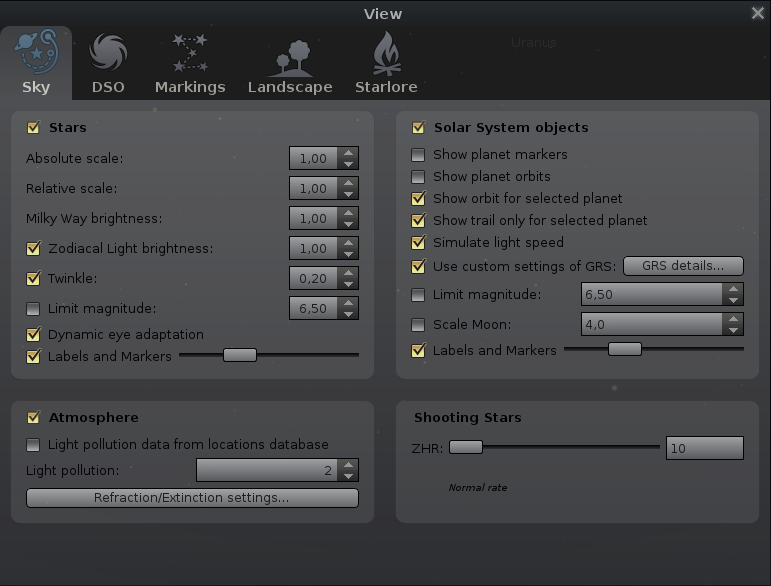
\includegraphics[scale=0.68]{view_dialog_sky_tab}
\caption{View Settings Window: Sky Tab}
\label{fig:viewwinskytab}
\end{figure}

The Sky tab of the View window (Fig.~\ref{fig:viewwinskytab}) contains settings
for changing the general appearane of the main sky view. Some
hightlights:

\begin{description}
\item[Absolute scale] is the size of stars as rendered by
  Stellarium. If you increase this value, all stars will appear larger
  than before.
\item[Relative scale] determines the difference in size of bright
  stars compared to faint stars. Values higher than 1.00 will make the
  brightest stars appear much larger than they do in the sky. This is
  useful for creating star charts, or when learning the basic
  constellations.
\item[Twinkle] controls how much the stars twinkle.
\item[Dynamic eye adaptation] When enabled this feature reduces the
  brightness of faint objects when a bright object is in the field of
  view. This simulates how the eye can be dazzled by a bright object
  such as the moon, making it harder to see faint stars and galaxies.
\item[Light pollution] In urban and suburban areas, the sky is
  brightned by terrestrial light pollution reflected in the atmophere.
  Stellarium simulates light pollution and is calibrated to the
  \emph{Bortle Dark Sky Scale} where 1 means a good dark sky, and 9 is
  a very badly light-polluted sky. See Appendix~\ref{ch:BortleScale}
  for more information.
\item[Planets and satellites] this group of options lets you turn on
  and off various features related to the planets. Simulation of light
  speed will give more precise positions for planetary bodies which move
  rapidly against backround stars (e.g. the moons of Jupiter). The
  \emph{Scale Moon} option will increase the apparent size of the moon
  in the sky, which can be nice for wide field of view shots.
\item[Labels and markers] you can independantly change the amount of
  labels displayed for planets, stars and nebuulae. The further to the
  right the sliders are set, the more labels you will see. Note that
  more labels will also appear as you zoom in.
\item[Shooting stars] Stellarium has a simple meteor simulation
  option. This setting controls how many shooting stars will be shown.
  Note that shooting stars are only visible when the time rate is 1, and
  might not be visiable at some times of day. Meteor showers are not
  currently simulated.
\end{description}



\subsection{Markings Tab}\label{marking-tab}

\begin{figure}[h]
\centering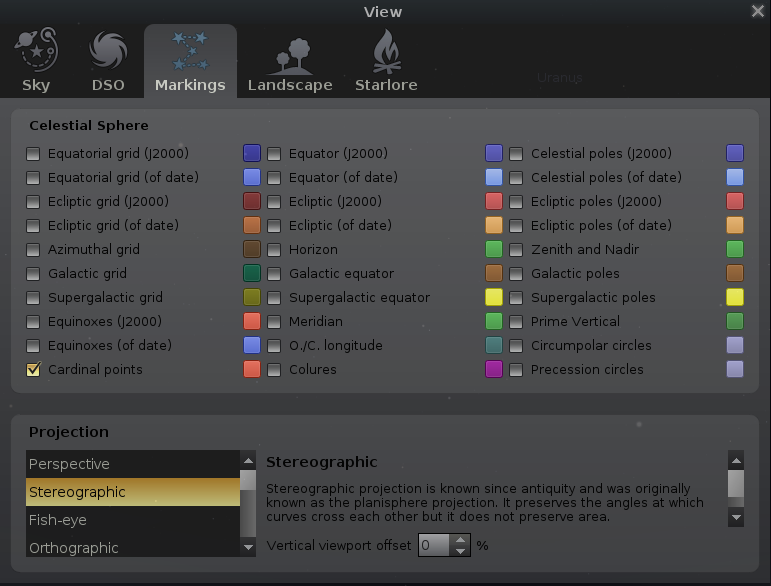
\includegraphics[scale=0.68]{view_dialog_markings_tab}
%\caption{Figure caption}
\end{figure}

The Markings tab of the View window controls the following features:

\begin{description}
\item[Celestial sphere] this group of options makes it possible to
  plot various grids and lines in the main view.
\item[Constellations] these controls let you turn on and off
  constellation lines, names, art and boundaries, and control the
  brightness of the constellation artwork.
\item[Projection] Selecting items in this list changes the
  projection method which Stellarium uses to draw the sky. Options are:

  \begin{description}
  \item[cylinder] The full name of this projection mode is
    \emph{cylindrical equidistant projection}. The maximum field of view
    in this mode is 233\degree.
  \item[equal area] The full name of this projection method is,
    \emph{Lambert azimuthal equal-area projection}. The maximum field of
    view is 360\degree.
  \item[fish-eye] Stellarium draws the sky using \emph{azimuthal
    equidistant projection}. In fish-eye projection, straight lines
    become curves when they appear a large angular distance from the
    centre of the field of view (like the distortions seen with very
    wide angle camera lenses). This is more pronounced as the user zooms
    out. The maximum field of view in this mode is 180\degree.
  \item[Hammer-Aitoff] The Hammer projection is an equal-area map
    projection, described by Ernst Hammer in 1892 and directly inspired
    by the Aitoff projection. The maximum field of view in this mode is
    360\degree.
  \item[mercator] Mercator projection preserves the angles between
    objects, and the scale around an object the same in all directions.
    The maximum field of view in this mode is 233\degree.
  \item[orthographic] Orthographic projection is related to
    perspective projection, but the \emph{point of perspective} is set
    to an infinite distance. The maximum field of view is 180\degree.
  \item[perspective] Perspective projection keeps the horizon a
    straight line. The maximum field of view is 150\degree. The mathematical
    name for this projection method is \emph{gnomonic projection}.
  \item[stereographic] This mode is similar to fish-eye projection
    mode. The maximum field of view in this mode is 235\degree.
  \end{description}
\end{description}

\subsection{Landscape Tab}\label{landscape-tab}

\begin{figure}[h]
\centering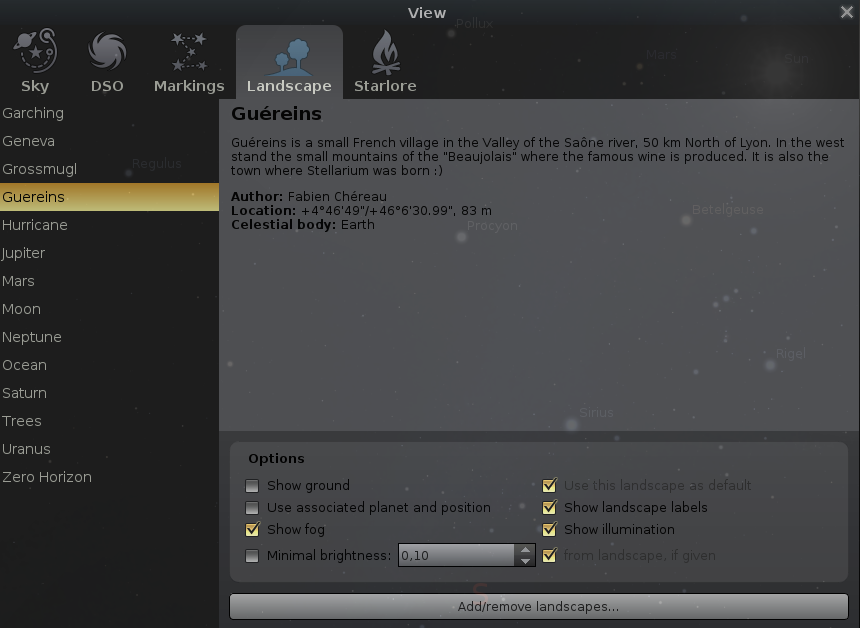
\includegraphics[scale=0.68]{view_dialog_landscape_tab}
%\caption{Figure caption}
\end{figure}

The Landscape tab of the View window controls the landscape graphics
(ground). To change the landscape graphics, select a landscape from the
list on the left side of the window. A description of the landscape will
be shown on the right.

Note that while landscape can include information about where the
landscape graphics were taken (planet, longitude, latitude and
altitude), this location does not have to be the same as the location
selected in the Location window, although you can set up Stellarium such
that selection of a new landscape will alter the location for you.

The controls at the bottom right of the window operate as follows:

\begin{description}
\item[Show ground] This turns on and off landscape rendering (same
  as the button in the main tool-bar).
\item[Show\_fog] This turns on and off rendering of a band of
  fog/haze along the horizon.
\item[Use associated planet and position] When enabled, selecting a
  new landscape will automatically update the observer location.
\item[Use this landscape as default] Selecting this option will save
  the landscape into the program configuration file so that the current
  landscape will be the one used when Stellarium starts.
\end{description}

\subsubsection{Starlore Tab}\label{starlore-tab}

\begin{figure}[h]
\centering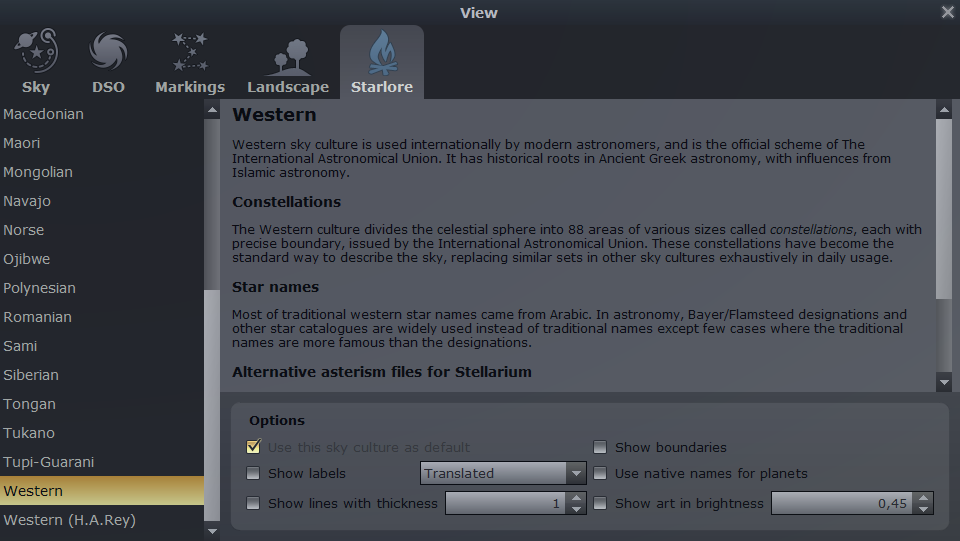
\includegraphics[scale=0.68]{view_dialog_starlore_tab}
%\caption{Figure caption}
\end{figure}

The Starlore tab of the View window controls what culture's
constellations and bright star names will be used in the main display.
Some cultures have constellation art (Western and Inuit), and the rest
do not.


\section{The Object Search Window}
\label{sec:gui:search}

\begin{figure}[h]
\centering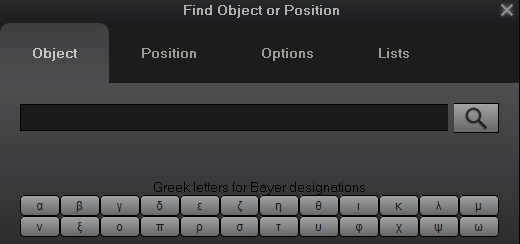
\includegraphics{search_dialog}
\caption{The Object Search Window}
\label{fig:gui:search}
\end{figure}

The Object Search window provides a convenient way to locate objects in
the sky. Simply type in the name of an object to find, and then click
the \button{go} button or press \key{return}. Stellarium will point you at that
object in the sky.

As you type, Stellarium will make a list of objects which begin with
what you have typed so far. The first of the list of matching objects
will be highlighted. If you press the \key{TAB} key, the selection will change
to the next item in the list. Hitting the \key{RETURN} key will go to the
currently highlighted object and close the search dialog.

For example, suppose we want to locate Mimas (a moon of Saturn). After
typing the first letter of the name, \emph{m}, Stellarium makes a list
of objects whose name begins with M: Mars, Mercury, Mimas, Miranda,
Moon. The first item in this list, Mars, is highlighted. Pressing \key{return}
now would go to Mars, but we want Mimas. We can either press \key{TAB} twice
to highlight Mimas and then hit \key{RETURN}, or we can continue to type the
name until it is the first/only object in the list.

\begin{figure}[h]
\centering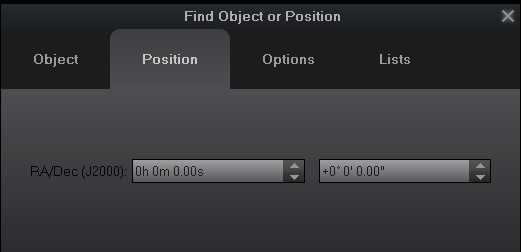
\includegraphics{search_dialog_position}
\caption{The Search Window: Positions}
\label{fig:gui:search:position}
\end{figure}

The Position tab provides a convenient way to enter a user set
of coordinates.

\begin{figure}[h]
\centering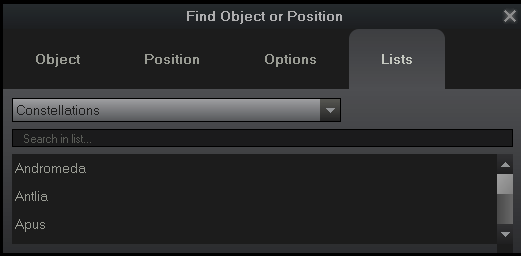
\includegraphics{search_dialog_list}
\caption{The Search Window: Lists}
\label{fig:gui:search:position}
\end{figure}

The List Search tab allows selection of an object from predefined
sets.  The number of choices is governed by the loaded plug
ins. Simply scroll down the first window to select the type. The name
of an object can then be selected from the list. Press \key{enter} and
stelarium will go to that object.


\begin{figure}[h]
\centering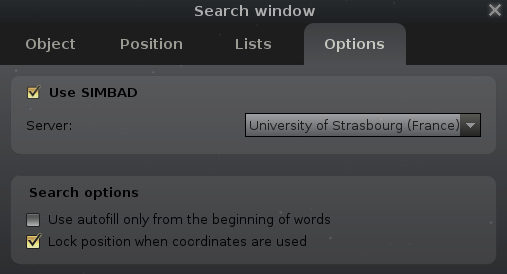
\includegraphics{search_dialog_option}
\caption{The Search Window: Options}
\label{fig:gui:search:options}
\end{figure}

The Options tab provides a few settings to fine-tune your search experience.
When the name of an object to find is typed in the object
window and you are connected to the internet and ``Extend search'' is
ticked, Stellarium will search the SIMBAD on-line  data bases for its
coordinates. You can then click the \button{go} button or press return.
Stellarium will point you at that object in the sky even if there is no
object displayed on the screen. The SIMBAD server being used can be
selected from the scroll window.


\section{Help Window}
\index{sec:gui:help}

\begin{figure}[h]
\centering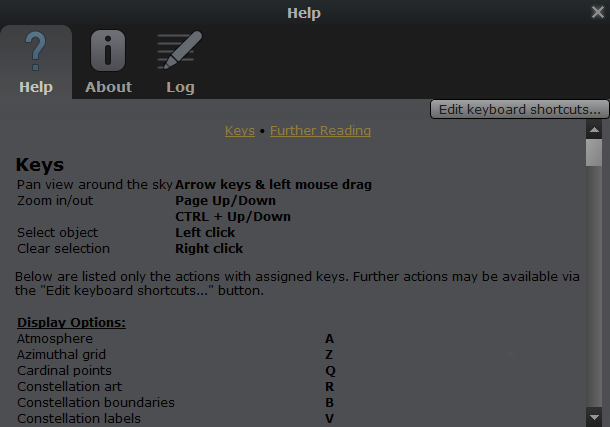
\includegraphics{help_dialog}
\caption{Help Window}
\label{fig:gui:help}
\end{figure}

The Help window lists all of Stellarium's key-strokes. Note that some
features are only available as key strokes, so it's a good idea to have
a browse of the information in this window.

\begin{figure}[h]
\centering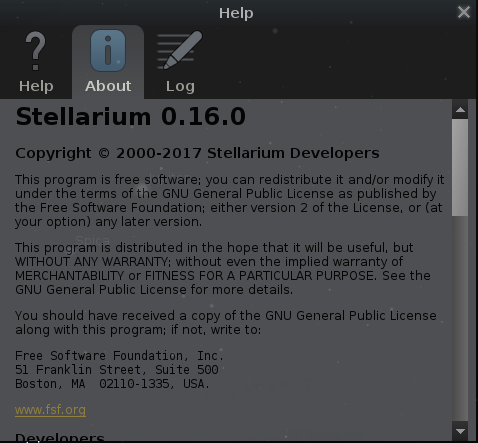
\includegraphics{help_dialog_about}
%\caption{Help Window}
\caption{Help Window: About}
\label{fig:gui:help:about}
\end{figure}

The About tab in this window will show licensing information, and a list
of people who helped to produce the program.

\begin{figure}[h]
\centering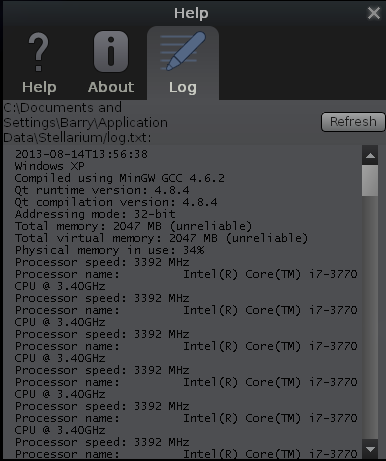
\includegraphics{help_dialog_log}
%\caption{Help Window}
\caption{Help Window: Logfile}
\label{fig:gui:help:log}
\end{figure}

The help window log tab shows the loading instructions carried out when
stellarium runs. It is useful to locate the files that stellarium writes
to your computer. The same information is written to  the file \file{log.txt} that you will
find in your user area (see~\ref{sec:Directories}).




%%% Local Variables: 
%%% mode: latex
%%% TeX-master: "guide"
%%% End: 
